\section*{Results}
So far, we have run some tests on randomly generated video sequences of whisker-like objects. While the results are far from good enough for practical use, they are still quite promising.

\begin{figure}
  \centering
  \begin{tabular}{ccc}
    
\includegraphics[width=0.3\textwidth]{tracking/frame10.png}
    & 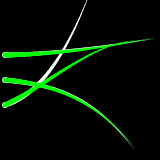
\includegraphics[width=0.3\textwidth]{tracking/frame20.png}
    & 
\includegraphics[width=0.3\textwidth]{tracking/frame30.png}
    \\
    Frame 10 & Frame 20 & Frame 30\\
    
\includegraphics[width=0.3\textwidth]{tracking/frame40.png}
    & 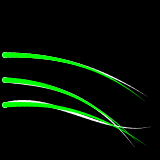
\includegraphics[width=0.3\textwidth]{tracking/frame50.png}
    & 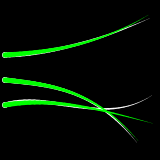
\includegraphics[width=0.3\textwidth]{tracking/frame60.png}
    \\
    Frame 40 & Frame 50 & Frame 60
  \end{tabular}

  \caption{Tracking result using 32 particles on 64 frames of generated whiskers. White is the whisker being tracked, green is the estimate of its position.}
  \label{fig:tracking}
\end{figure}

Figure \ref{fig:tracking} shows the tracking result on a sequence of 64 frames of generated, synthetic whiskers. The estimate of the whiskers' positions are at times close to perfect, but the tracking of the bottom whisker fails most of the time. Still, this illustrates the power of the probabilistic approach since this was run using only 32 particles, which is a very low amount. A 2.83 GHz Intel\textregistered \; Core\texttrademark \; 2 Quad computer system with 3.8 GiB of RAM running Ubuntu 10.04 running the tracker with 128 particles takes a little more than 4 seconds per frame and whisker, running on a single core.

\subsection*{Conclusions}
Our results so far lead us to believe that that it is indeed feasible to use this method for tracking whiskers.
